\chapter{Analisis dan Perancangan} \label{design-chapter}

\section{Analisis Masalah}\label{section-problem-analysis}

Digunakan teknik neural parametrik untuk membangkitkan suara alat musik gesek. Hal ini karena penggabungan komponen-komponen CSEMP alat musik gesek yang ada tidak memungkinkan karena masalah kompatibilitas. Selain itu, terdapat beberapa kemiripan dengan penerapan teknik neural parametrik untuk sintesis suara nyanyian dari sisi kontinuitas eksitasi dan jumlah not pada satu waktu. Teknik neural parametrik juga lebih baik dari sisi waktu eksekusi dibandingkan dengan teknik pembangkitan \textit{waveform} secara langsung. Untuk teknik neural parametrik ini, terdapat beberapa perbedaan masalah dengan penelitian sebelumnya\parencite{bonada2017singing}. Perbedaan masalah yang terjadi terdapat pada karakteristik suara alat musik, data input untuk sintesis, \textit{timing}. Perbedaan masalah-masalah ini adalah:

\begin{enumerate}

\item Perbedaan karakteristik suara alat musik gesek dan suara nyanyian terletak pada cara produksi suara dan gaung. Suara nyanyian memiliki gaung yang sedikit, sehingga tidak terdapat polifoni yang signifikan. Pada alat musik gesek, gaung sangat banyak digunakan sebagai bentuk ekspresi, sehingga terjadi polifoni akibat gaung. Selain itu, terdapat gaung yang secara intrinsik selalu muncul dari badan alat musik dan mempengaruhi warna suara.

\item \textit{Timing} not dalam alat musik gesek memiliki karakteristik yang berbeda dengan suara nyanyian. Dalam sistem \textit{baseline} untuk suara nyanyian, terdapat \textit{timing} fonetik. Dalam sistem ini, tidak ada \textit{timing} fonetik. Hanya dibutuhkan \textit{timing} not saja.

\item Perbedaan masalah untuk data input sintesis terkait dengan \textit{timbre}. Dalam pembangkitan suara alat musik gesek, \textit{timbre} ditentukan oleh konteks. Hal ini berbeda dengan penelitian sebelumnya, di mana \textit{timbre} ditentukan dari rangkaian fonem yang terdapat dalam data input.

\end{enumerate}

\section{Rancangan Umum Sistem}

Arsitektur sistem perbaikan terlihat pada Gambar \ref{fig-system-overview}, sebagai modifikasi dari Gambar \ref{fig-system-overview-bonada}. \ref{tab-models-in-out} Untuk menerapkan sistem yang dijelaskan pada Subbab \ref{literature-neural-parametric} ke alat musik gesek agar dapat dijalankan dan menghasilkan suara alat musik gesek, Dilakukan beberapa penyesuaian agar masalah-masalah pada Subbab \ref{section-problem-analysis} dapat diatasi:

\begin{enumerate}

    \item Perbedaan karakteristik suara alat musik diatasi dengan mengganti \textit{vocoder} dengan teknik pengkodean suara yang sesuai dengan alat musik gesek
    \item Aspek fonetik ditiadakan dari data \textit{timing} dan masukan kontrol untuk model \textit{timbre}
    \item Agar penentuan \textit{timbre} mempertimbangkan konteks, masukan model \textit{timbre} ditambahkan dengan masukan partitur dan \textit{timing} not

\end{enumerate}

Dalam sistem ini, pengkodean dan sintesis suara audio tidak dilakukan dengan \textit{vocoder} WORLD. Pengkodean dan sintesis suara audio dilakukan dengan pengkodean harmonik terarah plus stokastik dan sintesis harmonik plus stokastik. Teknik ini diharapkan  lebih cocok dengan karakteristik alat musik gesek dan mampu mengatasi adanya gaung.

Dalam sistem ini, seperti pada sistem pembangkit nyanyian, memiliki tiga model yang dilatih dengan data latih. Model-model itu adalah model \textit{timing}, model \textit{pitch}, dan model \textit{timbre}. Masukan dan keluaran setiap model tertulis pada Tabel \ref{tab-models-in-out}

Model \textit{timing} dalam sistem ini dilatih menggunakan partitur dan \textit{timing} not. Dengan demikian, diharapkan model \textit{timing} dapat memprediksi \textit{timing} dari not dalam partitur.

Model \textit{pitch} dalam sistem ini dilatih untuk menghasilkan F0. Masukan model ini adalah partitur dan \textit{timing}. Dalam pelatihan, masukan partitur dan \textit{timing} not diambil dari data latih, dan parameter \textit{vocoder} diambil dari hasil pengkodean harmonik terarah plus stokastik terhadap audio.

\begin{figure}[h]
    \centering
    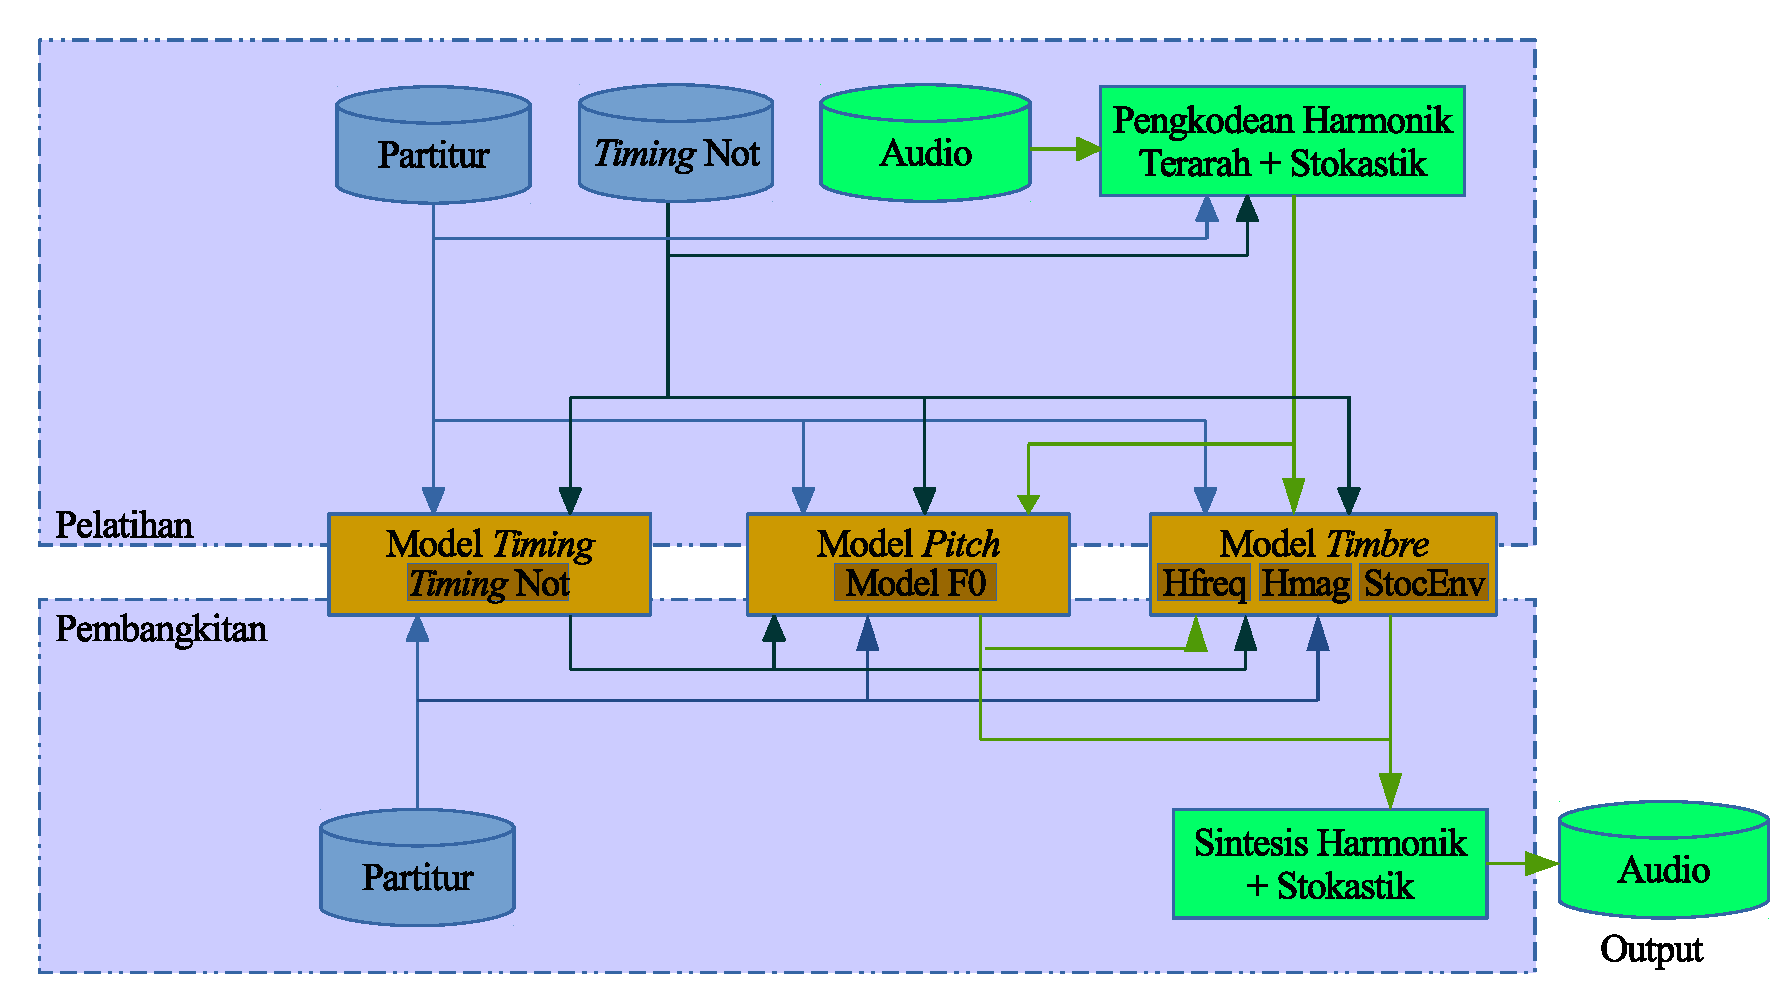
\includegraphics[width=0.8\textwidth]{resources/system-overview.eps}
    \caption{Adopsi teknik neural parametrik untuk permainan musik ekspresif alat musik gesek (modifikasi Gambar \ref{fig-system-overview-bonada})}\label{fig-system-overview}
\end{figure}

Pada tahap pembangkitan, sistem ini mampu menerima partitur dan menghasilkan audio. Keluaran perantara yang dihasilkan adalah parameter \textit{vocoder}, yang kemudian digunakan oleh \textit{vocoder} untuk menghasilkan audio.

Hal pertama yang dilakukan dalam tahap pembangkitan adalah prediksi \textit{timing} not. Setelah itu, partitur dan \textit{timing} not digunakan untuk memprediksi \textit{pitch} dan \textit{timbre}, dengan model yang sesuai. Parameter \textit{pitch} dan parameter \textit{timbre} digunakan untuk sintesis \textit{vocoder}.

Tiap model dari model-model ini adalah model regresi. Untuk model \textit{timing}, digunakan jaringan syaraf tiruan \textit{feedforward}. Untuk model \textit{pitch} dan model \textit{timbre}, digunakan jaringan syaraf tiruan dengan konvolusi kausal terdilasi. Masukan dari jaringan syaraf tiruan ini terdiri dari masukan fitur akustik output waktu sebelumnya dan masukan kontrol.

Masukan kontrol jaringan syaraf tiruan ini berasal dari partitur dan dari \textit{timing}. Untuk model \textit{timing}, masukan kontrol hanya berasal dari partitur. Untuk model \textit{pitch} dan model \textit{timbre}, masukan kontrol berasal dari partitur dan berasal dari \textit{timing}.

Masukan dari partitur dapat menunjukkan kondisi sesaat dan konteks. Kondisi sesaat berupa \textit{pitch} asli, panjang not, dan waktu dalam not. Kondisi konteks dapat berupa not sebelum dan sesudah, kunci, interval nada terhadap kunci, \textit{beat strength}, ataupun kondisi-kondisi lainnya hasil analisis karya. Namun, kakas analisis karya mungkin tida digunakan karena riset terkait analisis karya menggunakan komputer masih minim.

\begin{table}[h]
    \centering
    \caption{Masukan dan keluaran tiap model dalam sistem sintesis neural parametrik suara alat musik gesek }\label{tab-models-in-out}
    \begin{tabular}{ |c|c|c| } 
     \hline
     Model & Masukan & Keluaran \\
     \hline 
     Model \textit{timing} & partitur & \textit{timing} not  \\ 
     \hline
     Model \textit{pitch} & partitur & F0 \\ 
      & \textit{timing} not  & \\ 
     \hline
     Model \textit{timbre} & partitur   & Frekuensi harmonik \\ 
     & \textit{timing} not & Magnitudo harmonik\\
      & F0 & Amplop stokastik\\ 
     \hline
    \end{tabular}
\end{table}

\section{Pengkodean Harmonik Terarah Plus Stokastik}

Asumsi sumber eksitasi plus amplop spektral seperti yang digunakan pada \textit{vocoder} WORLD tidak dapat digunakan untuk alat musik gesek. Hal ini tampak pada hasil pengkodean menggunakan \textit{vocoder} WORLD dari data suara alat musik gesek yang telah dikumpulkan dengan cara yang dijelaskan pada Subbab \ref{datacollectionsection}.

Contoh hasil pengkodean dengan \textit{vocoder} WORLD tampak pada Gambar \ref{vocoderanalysisresultexample}. Pada gambar ini, tampak bahwa pada banyak bagian, \textit{vocoder} tidak dapat menyimpulkan frekuensi fundamental dari sinyal masukan. Begitu pula pada bagian amplop spektral dan aperiodistas, banyak bagian yang tidak dapat dideteksi amplop spektral dan aperiodisitasnya.

Hasil pengkodean seperti ini akan menghasilkan rekonstruksi sinyal yang jauh berbeda dibandingkan dengan sinyal masukan apabila dilakukan resintesis. Bahkan, pada banyak bagian, sinyal rekonstruksi tidak akan mengandung suara alat musik gesek sama sekali. Lebih lanjut, karena hasil pengkodean ini akan menjadi contoh keluaran untuk melatih model-model, model-model yang dilatih akan menghasilkan keluaran sebagaiman contoh yang diberikan pada data latih. Hasil sintesis dari keluaran model-model ini akan berbeda atau tidak mengandung suara alat musik gesek.

\begin{figure}[htbp]
    \centering
    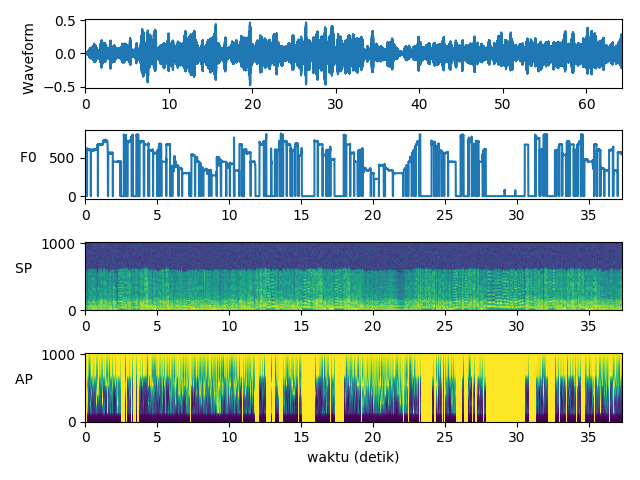
\includegraphics[width=\textwidth]{resources/Analisis_vocoder.png}
    \caption{Hasil pengkodean salah satu segmen data latih dengan \textit{vocoder} WORLD} \label{vocoderanalysisresultexample}
\end{figure}

Asumsi sumber eksitasi plus amplop spektral seperti yang digunakan pada \textit{vocoder} WORLD tidak dapat digunakan untuk alat musik gesek karena alat musik gesek menghasilkan suara dengan sumber eksitasi berupa gesekan antara \textit{bow} dan senar yang menghasilkan gelombang harmonik dan sedikit \textit{noise}, serta badan alat musik yang menghasilkan gaung. Selain badan alat musik, keberadaan beberapa senar juga memungkinkan gaung yang berasal dari senar-senar yang tidak sedang digesek.

Penentuan frekuensi fundamental pada \textit{vocoder} dengan memanfaatkan \textit{waveform}, misalnya dengan teknik \textit{zero-crossing interval}, mengasumsikan bahwa hanya terdapat satu sumber eksitasi. Karenanya, ketika terdapat gaung yang menyebabkan polifoni, \textit{zero-crossing interval} tidak dapat mendeteksi kemungkinan-kemungkinan frekuensi fundamental. Teknik DIO akan mendapati \textit{zero-crossing interval} yang tidak periodik sehingga ia tidak dapat menyimpulkan F0.

Berbeda dengan itu, teknik estimasi F0 dengan memanfaatkan puncak-puncak pada spektrum suara seperti TWM memilih F0 dari kandidat-kandidat dengan fungsi \textit{cost} tertentu. Karenanya, apabila pada satu \textit{frame} terdapat sinyal dari beberapa sumber suara, ia tetap dapat menyimpulkan beberapa kandidat F0 dan memilih salah satu di antaranya.

Agar penentuan frekuensi fundamental dari kandidat-kandidat frekuensi fundamental tidak dipengaruhi oleh gaung, pendeteksian frekuensi fundamental pada tiap langkah waktu dibatasi pada sekitar kemungkinan frekuensi fundamental not yang sedang dibunyikan pada langkah waktu tersebut. Untuk itu, diasumsikan bahwa frekuensi fundamental not yang sedang dibunyikan berada di sekitar frekuensi standar not.

Pencarian frekuensi fundamental dilakukan dengan algoritma TWM dengan fungsi \textit{cost} yang disesuaikan dengan jarak terhadap frekuensi standar. Fungsi \textit{cost} yang digunakan tampak pada persamaan berikut ini.

\begin{equation}
  TWMError'(f0c) = \dfrac{TWMError(f0c)}{f_{gauss}(semitone(f0c);notenumber,1)}
\end{equation}

Di sini, $f0c$ adalah frekuensi kandidat. $semitone(f0c)$ adalah konversi $f0c$ ke skala \textit{semitone} sesuai dengan skala nomor nada MIDI. $notenumber$ adalah nomor nada untuk not pada \textit{frame} yang sedang di kodekan. $f_{gauss}$ adalah fungsi Gaussian seperti yang tertulis di Persamaan \ref{eq-gauss-func} \parencite{Walpole}. Pencarian frekuensi fundamental dengan cara ini mengasumsikan bahwa deviasi frekuensi fundamental --dalam skala \textit{semitone}-- berdistribusi Gaussian.

\begin{equation}
 f_{gauss}(x;\mu,\sigma) = \dfrac{1}{\sigma \sqrt{2\pi}}e^{\dfrac{-(x-\mu)^2}{2 \sigma^2}} \label{eq-gauss-func}
\end{equation}

Agar gaung tidak mempengaruhi estimasi timbre, asumsi gelombang glottal dan amplop spektral tidak digunakan. Suara alat musik gesek diasumsikan berupa kumpulan gelombang-gelombang sinusoidal pada frekuensi-frekuensi harmonik saja, dengan tiap harmonik memiliki kemungkinan pergeseran. Pada tiap langkah waktu, setelah ditemukan frekuensi fundamental pada langkah waktu tersebut, dilakukan estimasi frekuensi-frekuensi harmonik dan ukuran tiap harmonik. Adapun fase dari tiap gelombang harmonik diabaikan.

Sisa spektrum yang tidak dapat dikodekan dengan gelombang-gelombang sinusoidal pada tiap harmonik tersebut kemudian dikodekan dengan model stokastik. Model ini merepresentasikan aperiodisitas.

Dengan demikian, hasil pengkodean harmonik terarah plus stokastik memiliki format yang sama dengan pengkodean harmonik plus stokastik. Hasilnya berupa deskripsi frekuensi fundamental, frekuensi dan ukuran harmonik, dan stokastik untuk setiap langkah waktu. Yang membedakan keduanya adalah adanya batasan frekuensi fundamental yang diarahkan oleh data partitur dan \textit{timing}.

Pengkodean dengan cara ini mampu mengatasi polifoni yang diakibatkan oleh gaung. Polifoni yang diakibatkan karena dua atau lebih not berbunyi sekaligus tidak dapat diatasi dengan cara ini. Cara ini hanya mampu mengekstrak satu frekuensi fundamental dari setiap langkah waktu.

\begin{figure}[h]
    \centering
    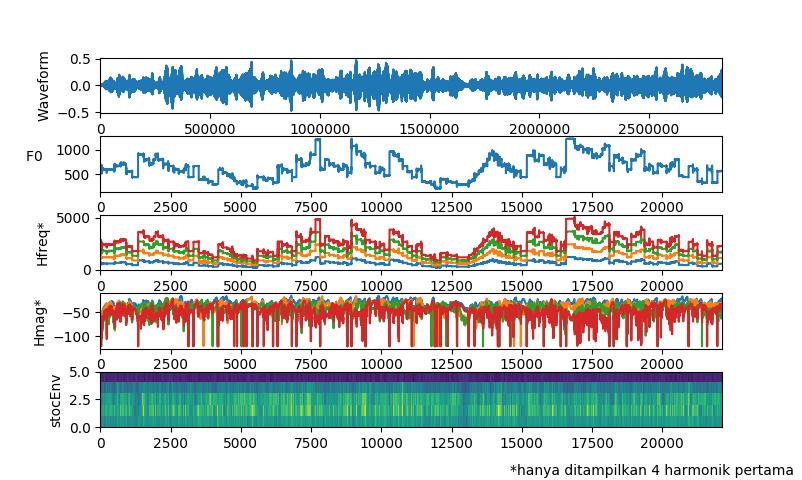
\includegraphics[width=\textwidth]{resources/Analisis_guidedtwmhps.png}
    \caption{Hasil pengkodean salah satu segmen data latih dengan pengkodean harmonik terarah plus stokastik} \label{guidedtwmhpsanalysisresultexample}
\end{figure}

Apabila dibandingkan dengan hasil pengkodean dengan \textit{vocoder} WORLD pada Gambar \ref{vocoderanalysisresultexample}, analisis harmonik terarah plus stokastik memiliki hasil pengkodean yang lebih baik. Gambar \ref{guidedtwmhpsanalysisresultexample} menunjukkan contoh hasil pengkodean dengan cara ini. Tampak bahwa data F0 dapat diperoleh dari keseluruhan keseluruhan sinyal.

\section{Model \textit{Timing}}

Model \textit{timing} berfungsi menentukan panjang aktual dari tiap not. Panjang aktual dari tiap not ini kemudian digunakan untuk menentukan waktu-waktu pergantian satu not ke not berikutnya.

\begin{figure}[htbp]
    \centering
    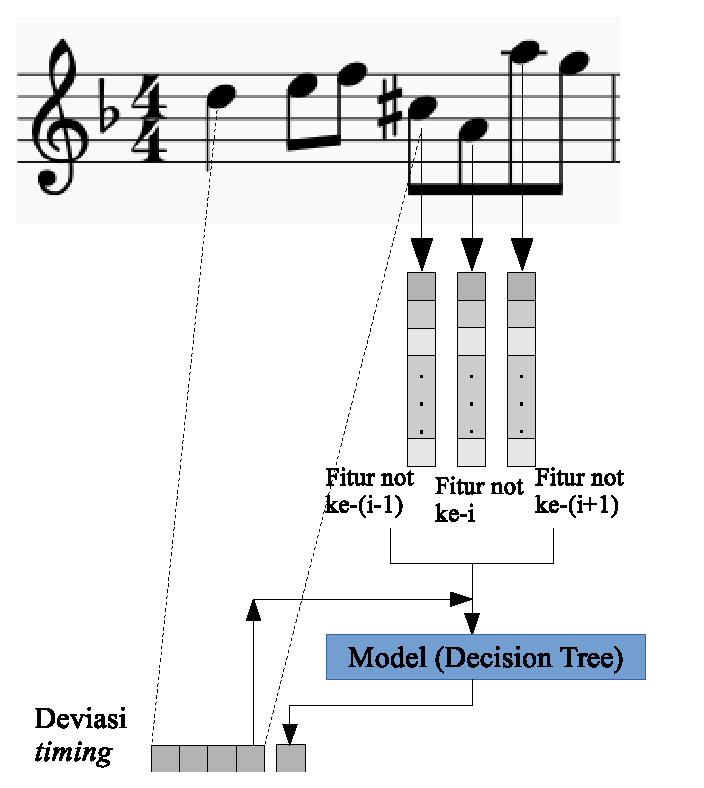
\includegraphics[width=0.9\textwidth]{resources/timing-model-in-out.eps}
    \caption{Input dan output model \textit{timing}}\label{fig-timing-model-in-out}
\end{figure}

Input dan output model \textit{timing} ditunjukkan pada Gambar \ref{fig-timing-model-in-out}. Deviasi \textit{timing} dibangkitkan satu per satu secara berurutan dari not awal hingga not akhir.

Model \textit{timing} dilatih dengan pasangan data latih fitur-fitur not dalam partitur dan \textit{timing} not tersebut. Keluaran yang diharapkan dari model ini adalah deviasi panjang not. Untuk tiap not, berikut ini adalah fitur-fitur not yang digunakan:

\begin{enumerate}
    \item panjang not yang tertulis dalam partitur
    \item panjang not sebelumnya yang tertulis dalam partitur
    \item posisi not dalam bar
    \item apakah not merupakan tanda istirahat
    \item apakah not sebelumnya merupakan tanda istirahat
    \item deviasi \textit{timing} not sebelumnya
\end{enumerate}

Apabila teknik neural parametrik nyanyian hendak diikuti, sebuah jaringan syaraf tiruan \textit{feedforward} terhubung penuh digunakan untuk membangun model \textit{timing}. Namun, terdapat perbedaan antara deviasi \textit{timing} pada nyanyian dengan deviasi \textit{timing} pada alat musik gesek. Permainan alat musik gesek memiliki \textit{range} deviasi \textit{timing} besar. Pada data yang dikumpulkan dengan langkah yang dijelaskan pada Subbab \ref{datacollectionsection}, \textit{range} deviasi \textit{timing} berkisar -4,44 s.d. 1,50 detik. Padahal, dengan arsitektur jaringan syaraf tiruan seperti model \textit{timing} nyanyian yang dijelaskan pada Subbab \ref{literature-neural-parametric}, \textit{range} deviasi \textit{timing} hanya dapat berkisar -0,15 s.d. 0,15 detik.

Apabila hendak digunakan jaringan syaraf tiruan dengan \textit{range} keluaran yang lebih besar, perlu dibuat model yang lebih kompleks. Padahal, data latih yang tersedia tidak cukup besar. Berbeda dengan model \textit{pitch} dan model \textit{timbre} dilatih \textit{frame} demi \textit{frame}, model \textit{timing} dilatih not demi not. Terdapat  1.064.100 \textit{frame} dalam data latih model \textit{pitch} dan model \textit{timbre}, sedangkan data latih model \textit{timing} hanya berisi 13.860 not dan tanda istirahat.

Dengan kondisi demikian, jaringan syaraf tiruan tidak akan mampu menangkap pola, dan mungkin hanya akan menganggap deviasi \textit{timing} sebagai \textit{noise}. Jaringan syaraf tiruan mungkin hanya akan merata-ratakan keluaran pada data latih. Teknik lain yang mampu mempelajari dari data yang berukuran kurang dari ukuran data ideal untuk jaringan syaraf tiruan, namun juga masih cukup kompleks, adalah \textit{decision tree}. Lebih lanjut, karena deviasi \textit{timing} berupa bilangan real, maka \textit{decision tree} yang digunakana adalah \textit{decision tree regression}, dengan fungsi impuritas yang biasa digunakan untuk masalah regresi yaitu \textit{mean squared error}.

\section{Model \textit{Pitch}}

Model \textit{pitch} berfungsi membangkitkan frekuensi fundamental untuk tiap langkah waktu. Digunakan jaringan syaraf tiruan dengan arsitektur yang sama dengan jaringan syaraf tiruan modifikasi Wavenet untuk sintesis neural parametrik nyanyan. Arsitektur ini tampak pada Gambar \ref{fig-network-architecture-bonada}.

\begin{figure}[htbp]
    \centering
    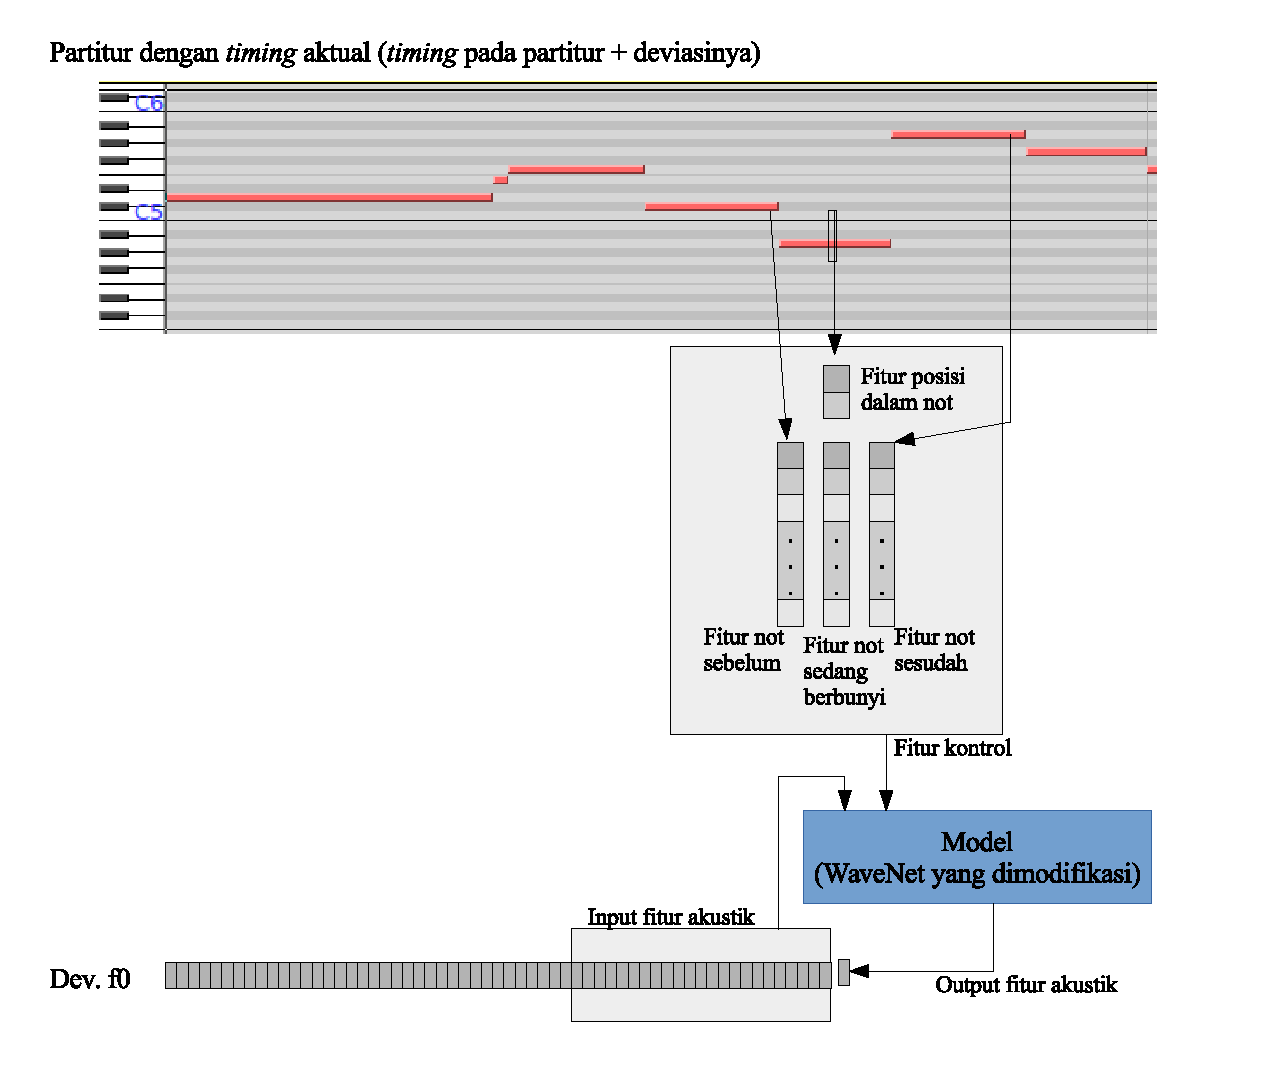
\includegraphics[width=0.9\textwidth]{resources/f0-model-in-out.eps}
    \caption{Input dan output model f0}\label{fig-f0-model-in-out}
\end{figure}

Input dan output model f0 ditunjukkan pada Gambar \ref{fig-f0-model-in-out}.tersebut. Deviasi f0 dibangkitkan satu per satu secara berurutan dari \textit{frame} awal hingga \textit{frame} akhir.

Input jaringan syaraf tiruan ini terdiri dari dua, yaitu input fitur akustik keluaran sebelumnya, dan input kontrol. Input kontrol berasal dari partitur.

Pembangkitan dilakukan untuk tiap langkah waktu secara berurutan dari depan ke belakang. Untuk tiap langkah waktu, keluaran dari beberapa langkah waktu sebelumnya, sepanjang medan reseptif, menjadi masukan pada langkah ini.

Fitur akustik yang dibangkitkan dan menjadi input fitur akustik berikutnya adalah deviasi f0, bukan f0 sebenarnya. Hal ini untuk menjaga konteks deviasi antar not. Deviasi f0 pada suatu not dipengaruhi oleh deviasi f0 pada not sebelumnya. Lebih lanjut, deviasi ini dihitung dalam skala logaritmik. Hubungan antara deviasi f0 dengan f0 ditunjukkan dalam Persamaan \ref{f0-deviation}, dengan $\Delta_{f_0}[t]$ adalah deviasi f0. Pada tahap pembangkitan, f0 dihitung dari persamaan ini.

\begin{equation}
    \Delta_{f_0}[t] = ln(f_0[t]) - ln({f_0}_{eq}(note[t]))
\end{equation}\label{f0-deviation}

Input kontrol yang digunakan berasal dari partitur dan estimasi \textit{timing} keluaran model \textit{timing}. Berdasarkan keluaran model \textit{timing}, dapat diketahui not pada partitur yang dibunyikan pada satu langkah waktu. Berdasarkan not tersebut, input kontrol ini terdiri dari fitur not tersebut, not sebelumnya, dan not sesudahnya. Fitur tiap not adalah sebagai berikut:

\begin{enumerate}
  \item nada tertulis absolut 
  \item durasi tertulis
  \item durasi aktual
  \item kunci tertulis (\textit{onehot})
  \item nada relatif terhadap kunci (\textit{onehot}, dalam 1 oktaf/12 \textit{semitone})
  \item not adalah \textit{grace}
  \item not memiliki tanda \textit{trill}
  \item tanda istirahat
  \item bukan tanda istirahat (not)
  \item posisi not dalam bar
  \item \textit{beat strength}
  \item \textit{quarter length}
\end{enumerate}

Selain itu, terdapat pula fitur yang menyatakan posisi \textit{frame} dalam not yang sedang berbunyi:

\begin{enumerate}
    \item posisi absolut dalam not
    \item posisi dalam not, relatif terhadap panjang not
\end{enumerate}

\section{Model \textit{Timbre}}

Model \textit{timbre} berfungsi membangkitkan representasi \textit{timbre}. Serupa dengan model \textit{pitch}, representasi \textit{timbre} untuk tiap langkah waktu dibangkitkan dengan input fitur akustik keluaran langkah-langkah waktu sebelumnya dan input kontrol. Digunakan jaringan syaraf tiruan dengan arsitektur pada Gambar \ref{fig-network-architecture-bonada}.

Representasi \textit{timbre} yang menjadi keluaran dan input fitur akustik model ini adalah sebagai berikut:

\begin{enumerate}
    \item $\Delta ln(f_h)$: deviasi frekuensi harmonik ke-$h$ dalam skala logaritmik, untuk semua komponen harmonik
    \item $mag_h$: ukuran/magnitudo (desibel) komponen harmonik ke-$h$, untuk semua komponen harmonik
    \item $stoc_s$: ukuran komponen stokastik ke-$s$, disebut juga amplop stokastik
\end{enumerate}

\begin{figure}[htbp]
    \centering
    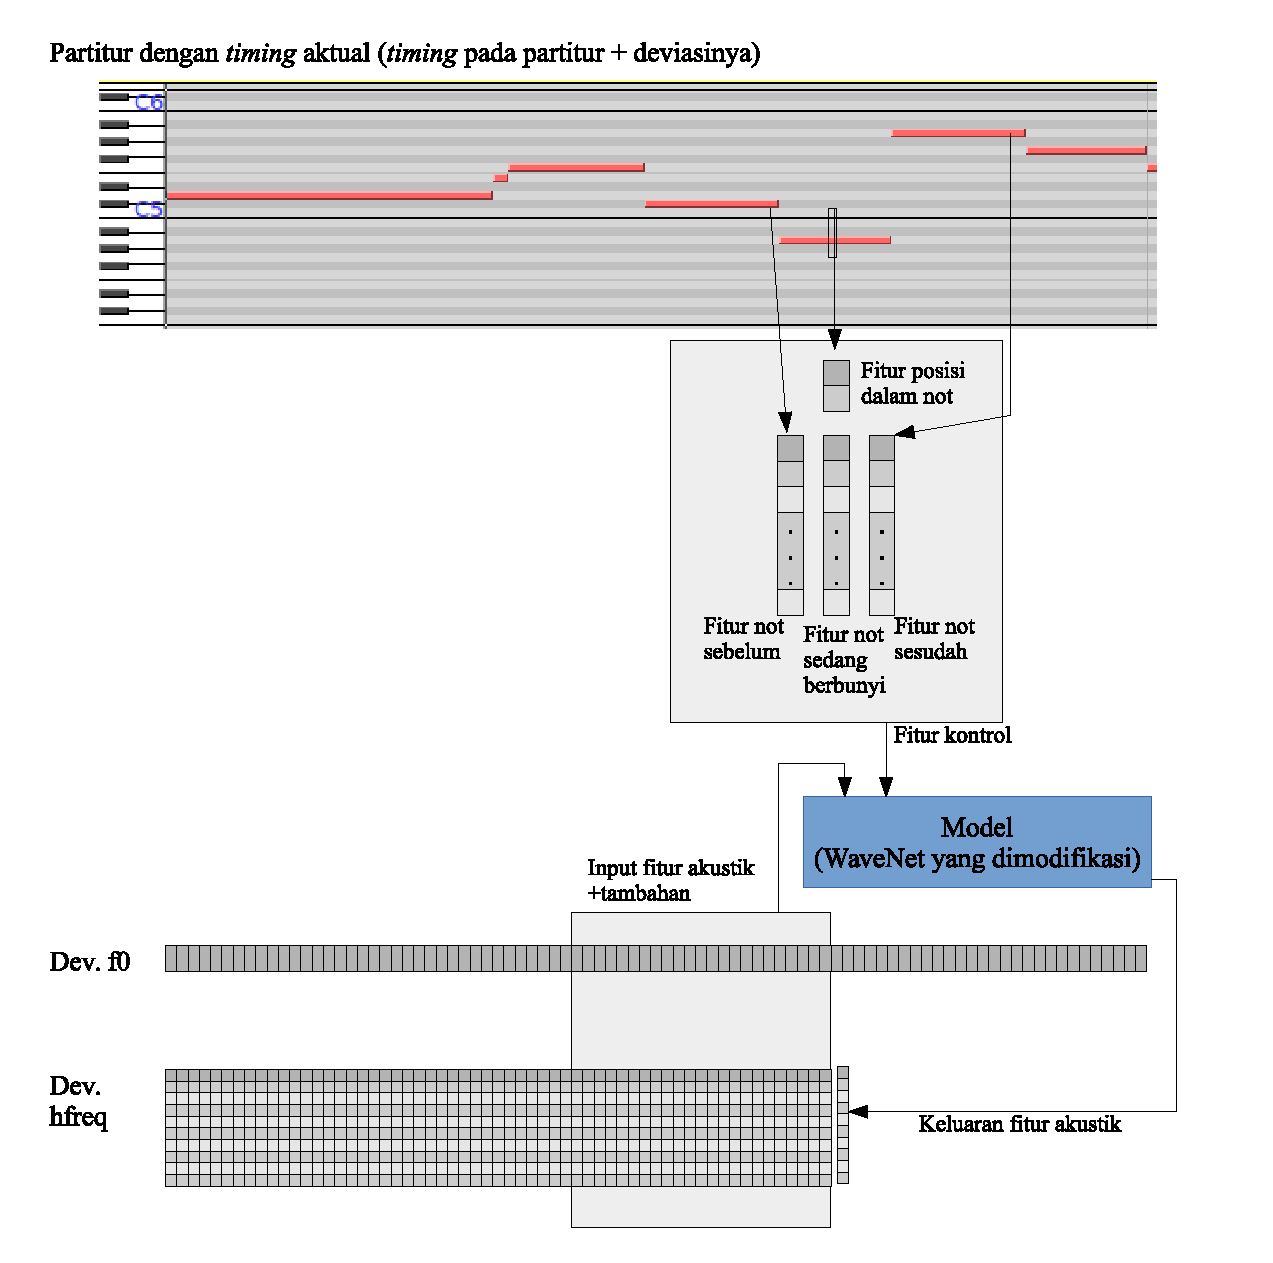
\includegraphics[width=0.9\textwidth]{resources/hfreq-model-in-out.eps}
    \caption{Input dan output model frekuensi harmonik}\label{fig-hfreq-model-in-out}
\end{figure}

Input dan output model frekuensi harmonik ditunjukkan pada Gambar \ref{fig-hfreq-model-in-out}. Deviasi frekuensi harmonik dibangkitkan satu per satu secara berurutan dari \textit{frame} awal hingga \textit{frame} akhir.

\begin{figure}[htbp]
    \centering
    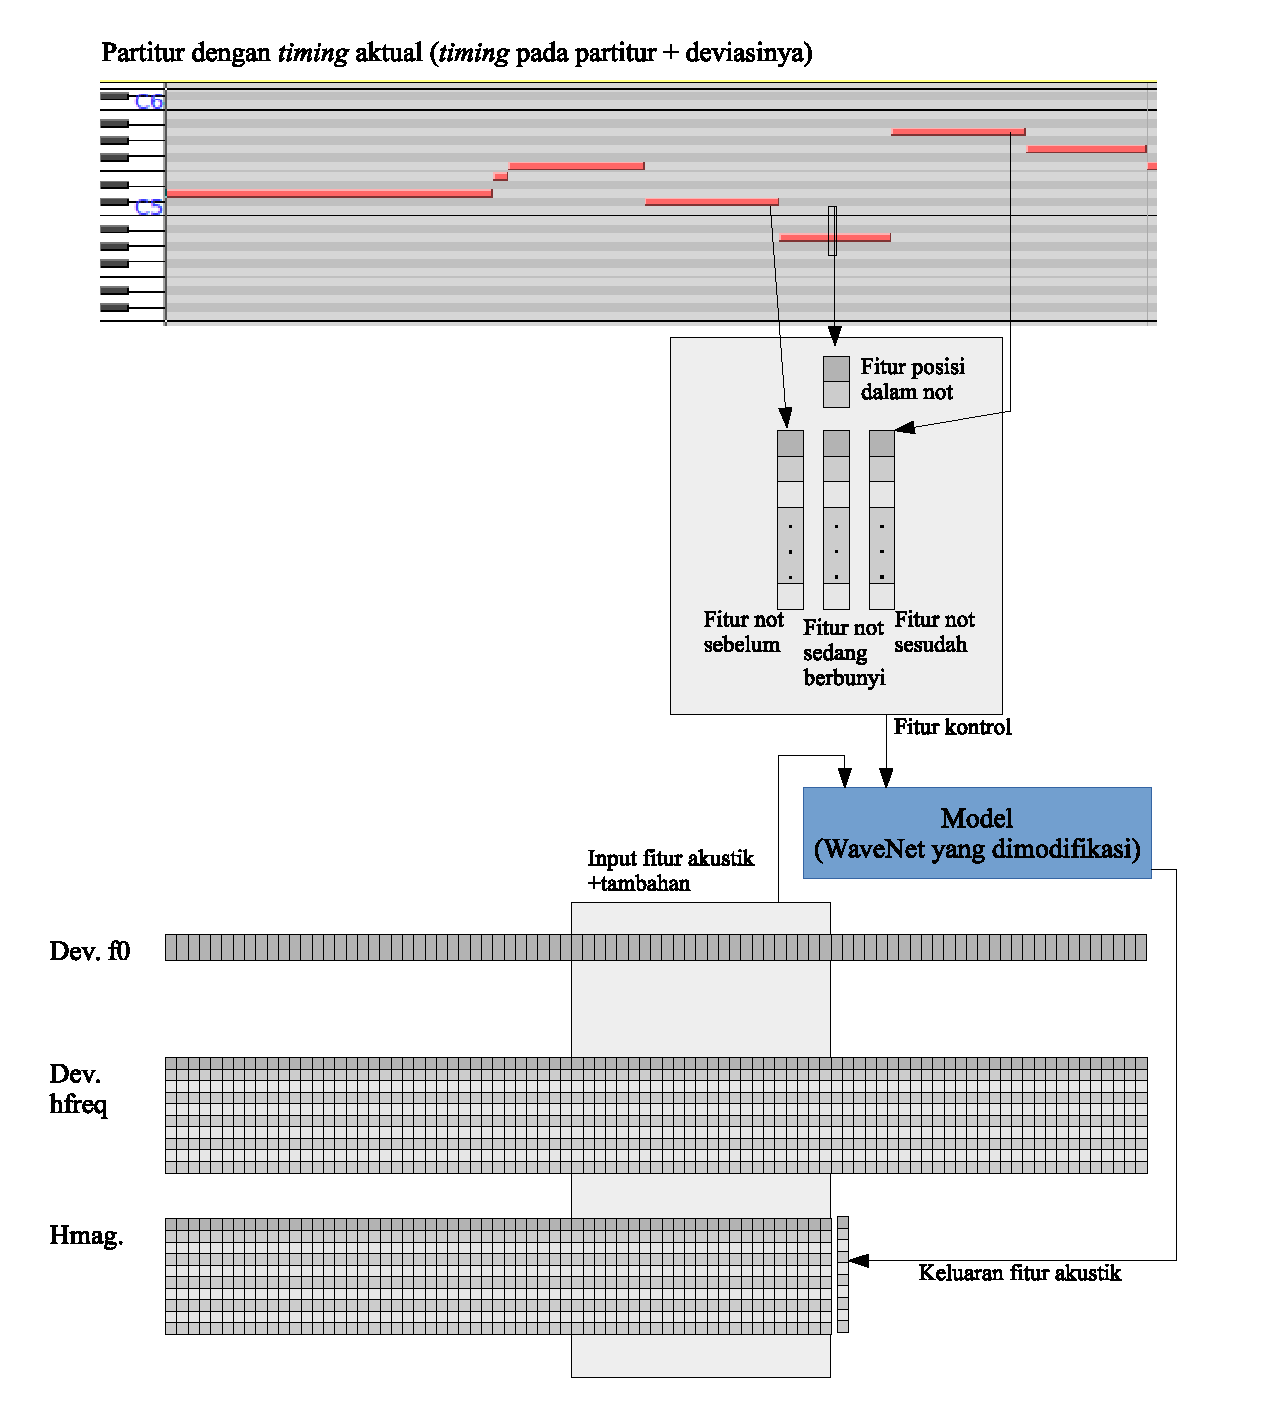
\includegraphics[width=0.9\textwidth]{resources/hmag-model-in-out.eps}
    \caption{Input dan output model magnitudo harmonik}\label{fig-hmag-model-in-out}
\end{figure}

Input dan output model magnitudo harmonik ditunjukkan pada Gambar \ref{fig-hmag-model-in-out}. Deviasi magnitudo harmonik dibangkitkan satu per satu secara berurutan dari \textit{frame} awal hingga \textit{frame} akhir.

\begin{figure}[htbp]
    \centering
    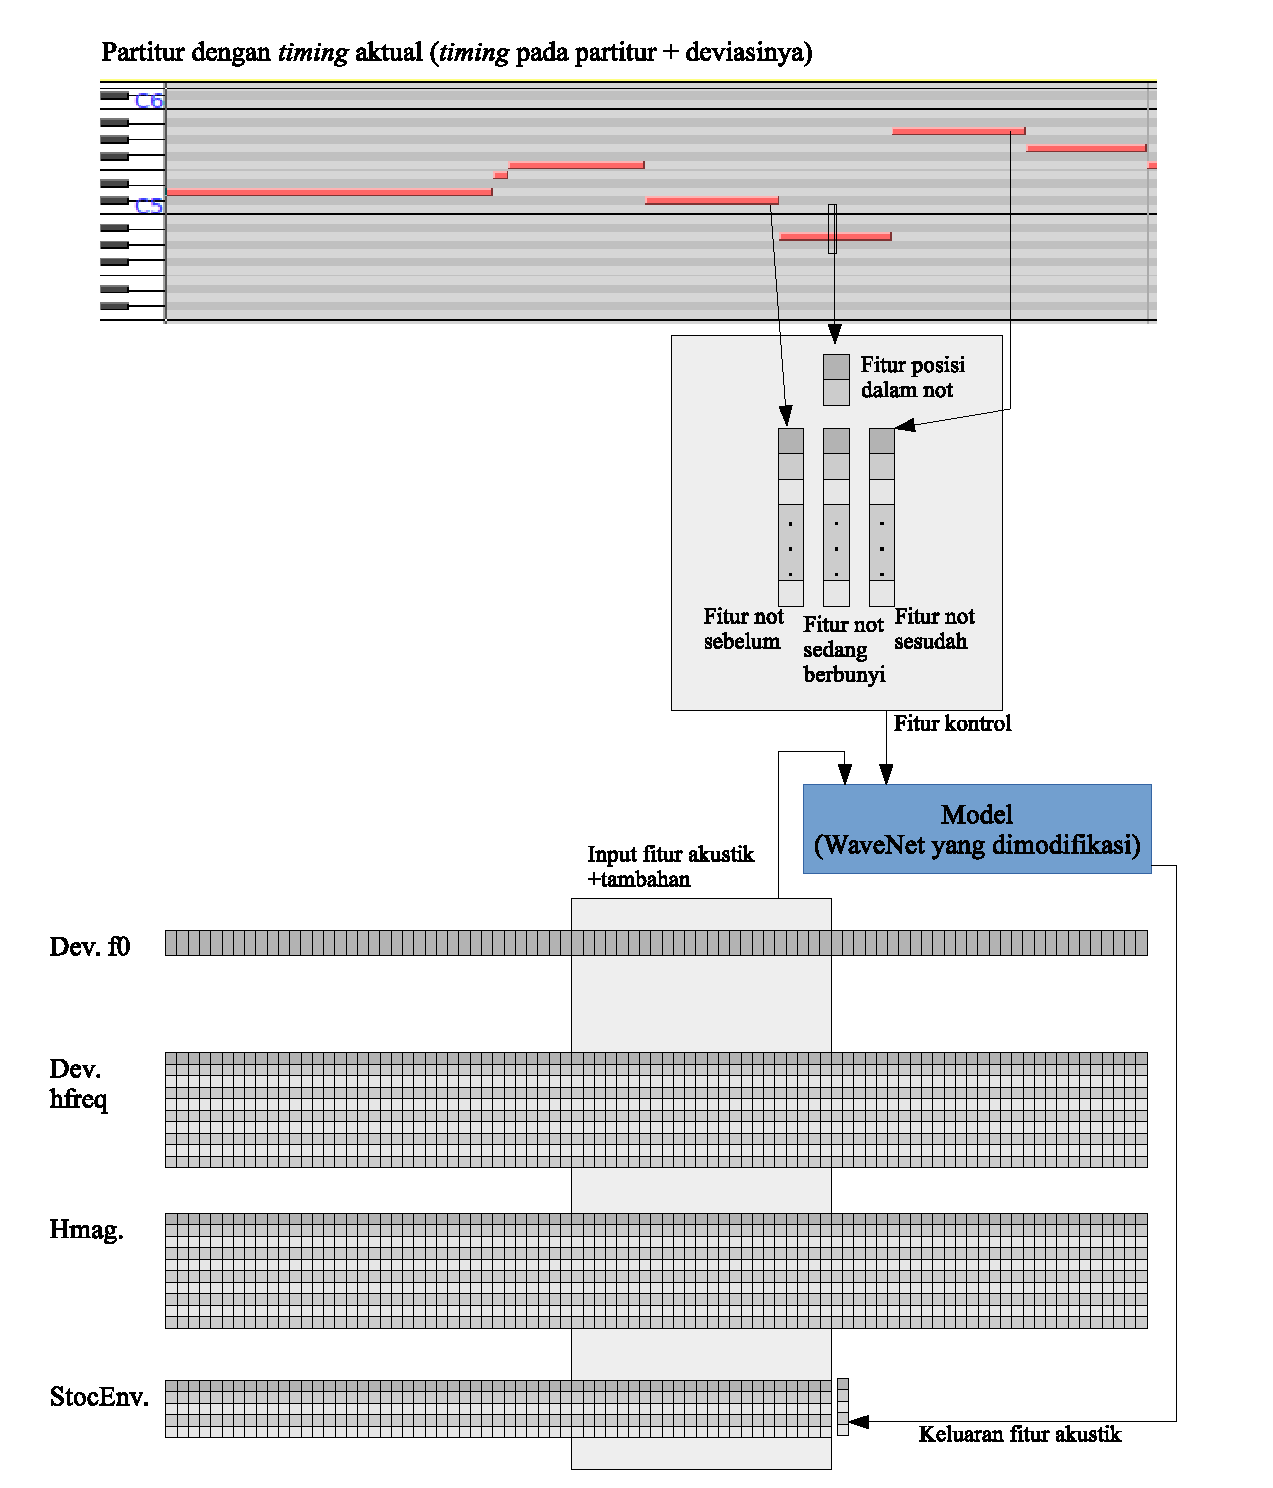
\includegraphics[width=0.9\textwidth]{resources/stocenv-model-in-out.eps}
    \caption{Input dan output model amplop stokastik}\label{fig-stocenv-model-in-out}
\end{figure}

Input dan output model amplop stokastik ditunjukkan pada Gambar \ref{fig-stocenv-model-in-out}. Deviasi amplop stokastik dibangkitkan satu per satu secara berurutan dari \textit{frame} awal hingga \textit{frame} akhir.

Input kontrol untuk model ini sama dengan input kontrol model \textit{pitch}. Input kontrol ini terdiri dari fitur-fitur not dan fitur not konteks. Fitur tiap not sama dengan fitur tiap not yang digunakan untuk model \textit{pitch}

Terdapat input tambahan yang dimasukkan bersama dengan input fitur akustik untuk tiap model bagian model timbre. Semua model-model bagian model \textit{pitch} mendapat input tambahan deviasi f0. Model frekuensi harmonik menerima input tambahan deviasi f0. Model magnitudo harmonik menerima input tambahan deviasi f0 dan deviasi frekuensi harmonik. Model amplop stokastik menerima input tambahan deviasi f0, deviasi frekuensi harmonik, dan magnitudo harmonik.

\section{Data Partitur, \textit{Timing}, dan Audio} \label{datacollectionsection}

Untuk melatih sistem ini, dibutuhkan data latih berupa partitur, \textit{timing} dan rekaman audio. Untuk itu, dibutuhkan partitur dan rekaman audio yang bersesuaian. Data dikumpulkan secara manual.

Partitur didapatkan dari Petrucci Music Library, dengan memilih secara berurutan dari daftar lagu untuk satu alat musik gesek. Dari daftar lagu tersebut, dipilih lagu yang dapat ditemukan rekaman audionya pada situs \textit{media sharing} publik.

Tidak semua lagu yang memiliki rekaman audio bersesuaian digunakan. Partitur dikumpulkan berurutan secara alfabetis dengan kriteria tidak memiliki gaung terlalu besar seperti gaung ruangan. Minimal total durasi seluruh data yang dikumpulkan adalah 30 menit. Minimal total durasi ini didasarkan kepada riset neural parametrik nyanyian.

Partitur terkumpul kemudian disalin dari format gambar atau PDF ke dalam format MusicXML. Penyalinan ke dalam format MusicXML dilakukan secara manual.

Karena pengkodean harmonik plus sinusoidal hanya mampu menghasilkan suara monofonik, maka partitur dan rekaman tersebut kemudian dipotong-potong ke segmen-segmen yang monofonik. Segmen-segmen polifonik tidak digunakan.

Data \textit{timing} dibuat dengan teknik DTW lalu diperbaiki secara manual dari rekaman audio. DTW dilakukan dengan fungsi \textit{cost} berupa jarak \textit{pitch} hasil deteksi f0 dengan TWM (tanpa arahan) terhadap \text{pitch} not yang tertulis dalam partitur, dalam skala \textit{semitone}. Transisi DTW dibatasi hanya ke arah lateral yaitu transisi \textit{frame}. Transisi ke arah vertikal yaitu transisi \textit{not} hanya dapat dilakukan bersamaan dengan transisi lateral. Pembatasan DTW ini tampak pada Gambar \ref{fig-dtw-transition}

\begin{figure}[htb]
    \centering
    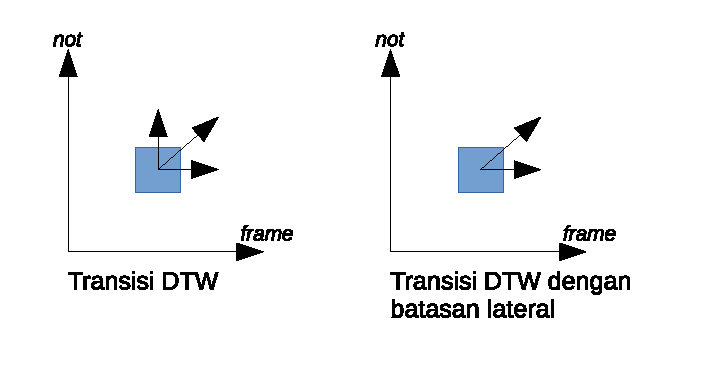
\includegraphics[width=0.8\textwidth]{resources/DTW-transition.eps}
    \caption{Pembatasan transisi DTW untuk ekstraksi data \textit{timing}}\label{fig-dtw-transition}
\end{figure}

Dengan didahului DTW tersebut, anotator hanya perlu mengoreksi keluaran dari DTW pada bagian-bagian yang salah. Anotator memperbaiki waktu-waktu perubahan not dengan cara mendengarkan rekaman suara, dibantu dengan tampilan spektogram. Gambar \ref{dtw-output-example} menunjukkan contoh keluaran DTW yang kemudian diperbaiki. Contoh perbaikan oleh anotator tampak pada Gambar \ref{dtw-output-example-corrected}. Bagian atas menunjukkan spektogram yang digunakan oleh anotator untuk memperbaiki \textit{timing}, dan bagian bawah menunjukkan \textit{timing} pergantian not.

\begin{figure}[htb]
  \centering
  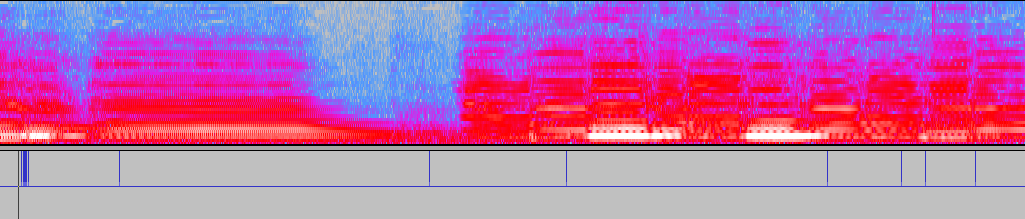
\includegraphics[width=0.8\textwidth]{resources/DTW-output-example.png}
  \caption{Contoh \textit{timing} pergantian not keluaran DTW yang memiliki kesalahan} \label{dtw-output-example}
\end{figure}

\begin{figure}[htb]
  \centering
  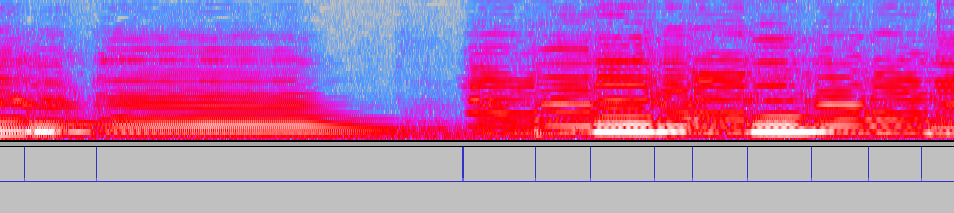
\includegraphics[width=0.8\textwidth]{resources/DTW-output-corrected-example.png}
  \caption{Contoh \textit{timing} pergantian not keluaran DTW yang telah diperbaiki anotator} \label{dtw-output-example-corrected}
\end{figure}

Untuk kebutuhan eksperimen, data yang dikumpulkan terdiri dari dua bagian. Bagian pertama, data latih, digunakan untuk melatih model. Data uji digunakan untuk menguji model.

\section{Skema Pemilihan Subset Data Latih}\label{subsetselectionsection}

Di antara masalah yang dihadapi untuk model-model dengan arsitektur \textit{wavenet} yang dimodifikasi adalah kinerjanya menurun apabila data latih ditambah lebih dari ukuran tertentu. Namun, pada riset neural parametrik nyanyian, tidak disebutkan komponen apa yang mengalami fenomena ini.

Untuk sintesis neural parametrik alat musik gesek, akan dilakukan pemilihan subset data latih untuk tiap model yang menggunakan arsitektur jaringan syaraf tiruan modifikasi WaveNet. Untuk efisiensi, kandidat subset yang digunakan adalah subset-subset yang juga digunakan pada validasi silang. Selain itu, keseluruhan data latih juga dijadikan kandidat.

Dari model-model yang telah dilatih dengan kandidat-kandidat subset tersebut, dipilih model yang memiliki kinerja tertinggi terhadap keseluruhan data latih. Hal ini didasarkan kepada dugaan bahwa model yang memiliki kinerja tinggi terhadap data latih akan memiliki kinerja tinggi juga kepada data uji. Dugaan ini didasari pada jumlah \textit{frame} yang cukup banyak pada data latih. Dugaan ini akan dibuktikan dengan eksperimen.

\section{Teknik Neural Parametrik sebagai Perencana Gestur Ekspresi}

Di antara kekurangan teknik jaringan syaraf tiruan adalah kemungkinannya tidak mampu mempelajari secara detil bentuk-bentuk dari keluaran model \textit{timbre}. Jaringan syaraf tiruan yang diajukan memiliki kecenderungan mendahulukan mempelajari pola jangka-panjang yang dan menganggap pola-pola jangka pendek seperti \textit{spike} dan \textit{vibrato} sebagai \textit{noise}. Padahal, bisa jadi pola-pola jangka pendek tersebut sangat mempengaruhi persepsi warna suara alat musik dan kealamiannya.

Selain pola jangka-pendek yang diabaikan oleh jaringan syaraf tiruan, terdapat masalah terkait perbedaan \textit{timbre} antara transisi not dan pertengahan not. Meskipun fitur untuk model \textit{timbre} meliputi juga posisi dalam not, namun jaringan syaraf tiruan mungkin saja akan mengeluarkan hasil yang sama untuk transisi not dan pertengahan not. Hal ini karena panjang bagian yang berbeda tersebut pada suatu not dan not lain mungkin berbeda-beda. Akibatnya, jaringan syaraf tiruan tidak mampu melihat batasan tersebut dan menganggap perbedaan bagian transisi dan pertengahan not sebagai \textit{noise} pada data. Hal ini juga mempengaruhi persepsi warna suara alat musik dan kealamiannya.

Untuk mengatasi hal tersebut, dapat digunakan teknik lain yang warna suara alat musiknya sudah cukup mirip dengan alat musik gesek, dan teknik neural parametrik digunakan untuk membangkitkan gestur ekspresi. Garis besar pendekatan ini terlihat di Gambar \ref{fig-dtnp-as-gesture-planner}. Keluaran sistem pensintesis neural parametrik alat gesek dikonversi menjadi gestur-gestur ekspresi berupa deviasi \textit{pitch} dan dinamika.

\begin{figure}[htb]
  \centering
  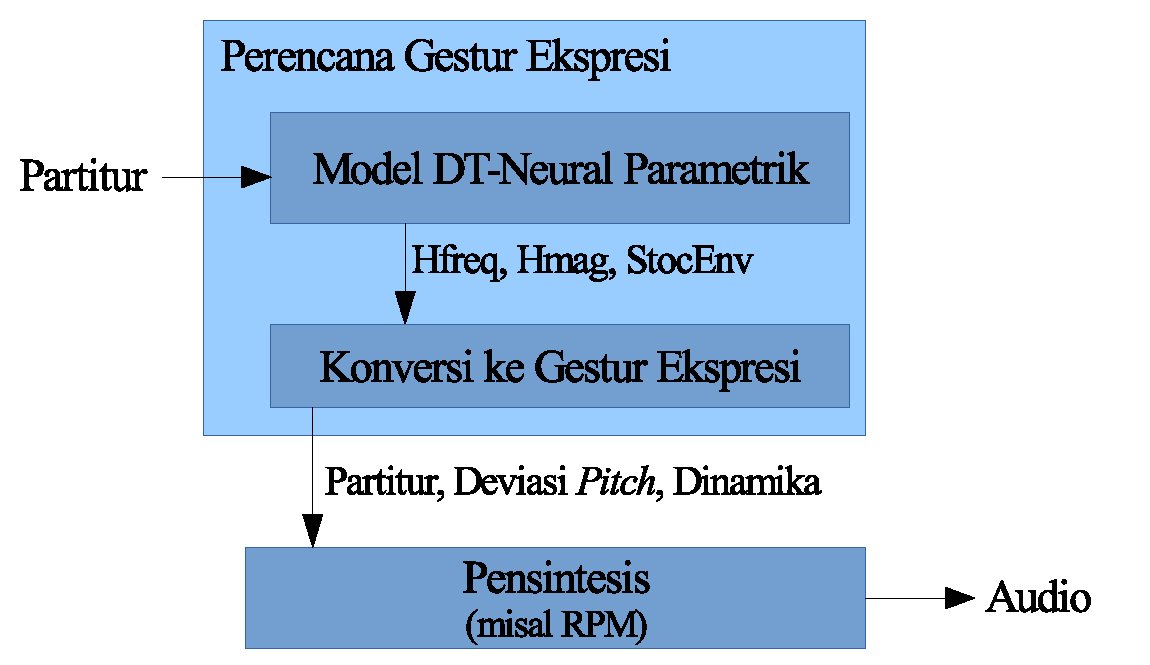
\includegraphics[width=\textwidth]{resources/DTNP-as-gesture-planner.eps}
  \caption{Penggunaan teknik neural parametrik untuk perencana gestur ekspresi}\label{fig-dtnp-as-gesture-planner}
\end{figure}

Deviasi \textit{pitch} diambil dari perbedaan antara \textit{pitch} keluaran model dan \textit{pitch} non-ekspresif yang tertulis dalam partitur. Perbedaan ini dihitung dalam skala \textit{semitone}. Dinamika dihitung dari keseluruhan magnitudo harmonik. Magnitudo total dari keseluruhan harmonik dihitung dengan cara menjumlahkan \textit{pressure/voltage level}.

Dengan pendekatan ini, tidak semua ekspresi yang dihasilkan oleh teknik neural parametrik dapat digunakan. Pensintesis yang ada hanya menerima gestur deviasi \textit{pitch} dan dinamika. Variasi \textit{timbre} tidak diteruskan ke pensintesis. Variasi \textit{timbre} hanya ditentukan oleh pensintesis.